%!TEX root = ../dissertation.tex

\chapter{Solution}
\label{chapter:solution}
This chapter proposes a solution to determine if the cloud is able to meet the fundamental requirements
of \gls{IoT} applications. As described in Chapter \ref{chapter:introduction}, we will follow two
approaches to deploy the smart warehouse application in the cloud, the cloud-based and the fog-based
approach. Furthermore, we also propose a mechanism to automate the provisioning of applications
middleware in the cloud.

% Smart Warehouse Deployment
\section{Smart Warehouse Deployment}
\label{sec:smart_warehouse_deployment}
As described in Section \ref{sub:domain}, our smart warehouse is composed of smart objects that
can be identified by readers and sensors that are placed in the warehouse. In traditional solutions,
the application is provisioned in a local infrastructure. Although this approach guarantees that
some fundamental requirements are fulfilled - such as the low-latency interaction - this solution
comes with several bottlenecks - such as the low scalability, infrastructure costs and maintenance -
that can be a barrier for those types of applications.\\

Leveraging the infrastructure required to provisioning the \gls{IoT} applications to the cloud
guarantees that some of the bottlenecks of traditional solutions are solved. However, we also need
to guarantee that the requirements of those applications are fulfilled. The following sections
describes the approaches to deploy the application in the cloud and to automate their
provisioning.

% Cloud approach
\subsection{Cloud Deployment}
\label{sub:sol_cloud}

% Cloud approach
\begin{figure}[ht!]
  \centering
  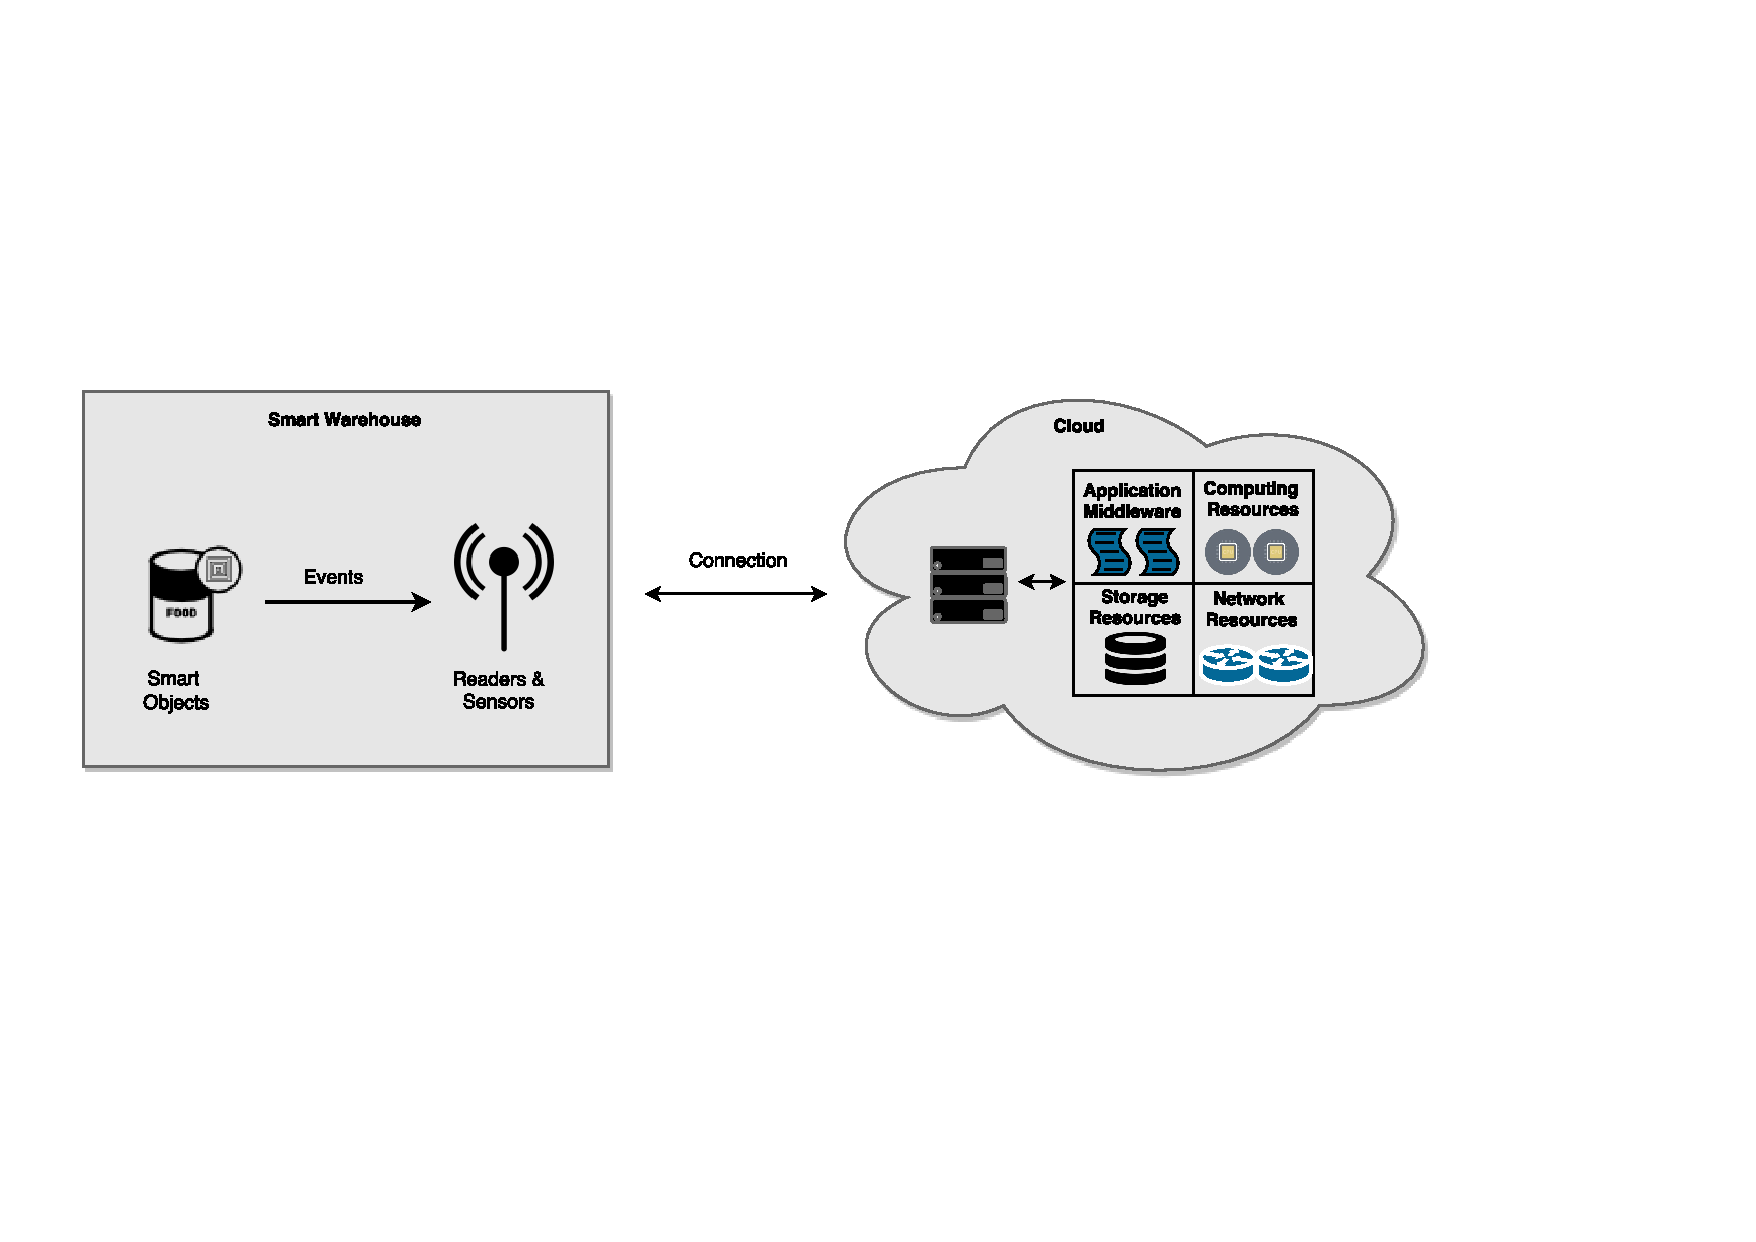
\includegraphics[width=\textwidth]{./images/solution_cloud_architecture}
  \caption{Cloud-approach: smart warehouse conceptual architecture.}
  \label{fig:solution_cloud_architecture}
\end{figure}

Figure~\ref{fig:solution_cloud_architecture} presents the architecture of a cloud-based smart warehouse.
The warehouse is composed of smart objects, sensors and readers that capture the events that occurs
in the warehouse. The application middleware is provisioned in the cloud, which virtualizes the computing,
storage and network resources needed to support the application.\\

The smart warehouse is connected to the cloud through a wireless connection such as Wi-Fi, 3G or
\gls{LTE}.

% Fog approach
\subsection{Fog Deployment}
\label{sub:sol_fog}

% Fog approach
\begin{figure}[ht!]
  \centering
  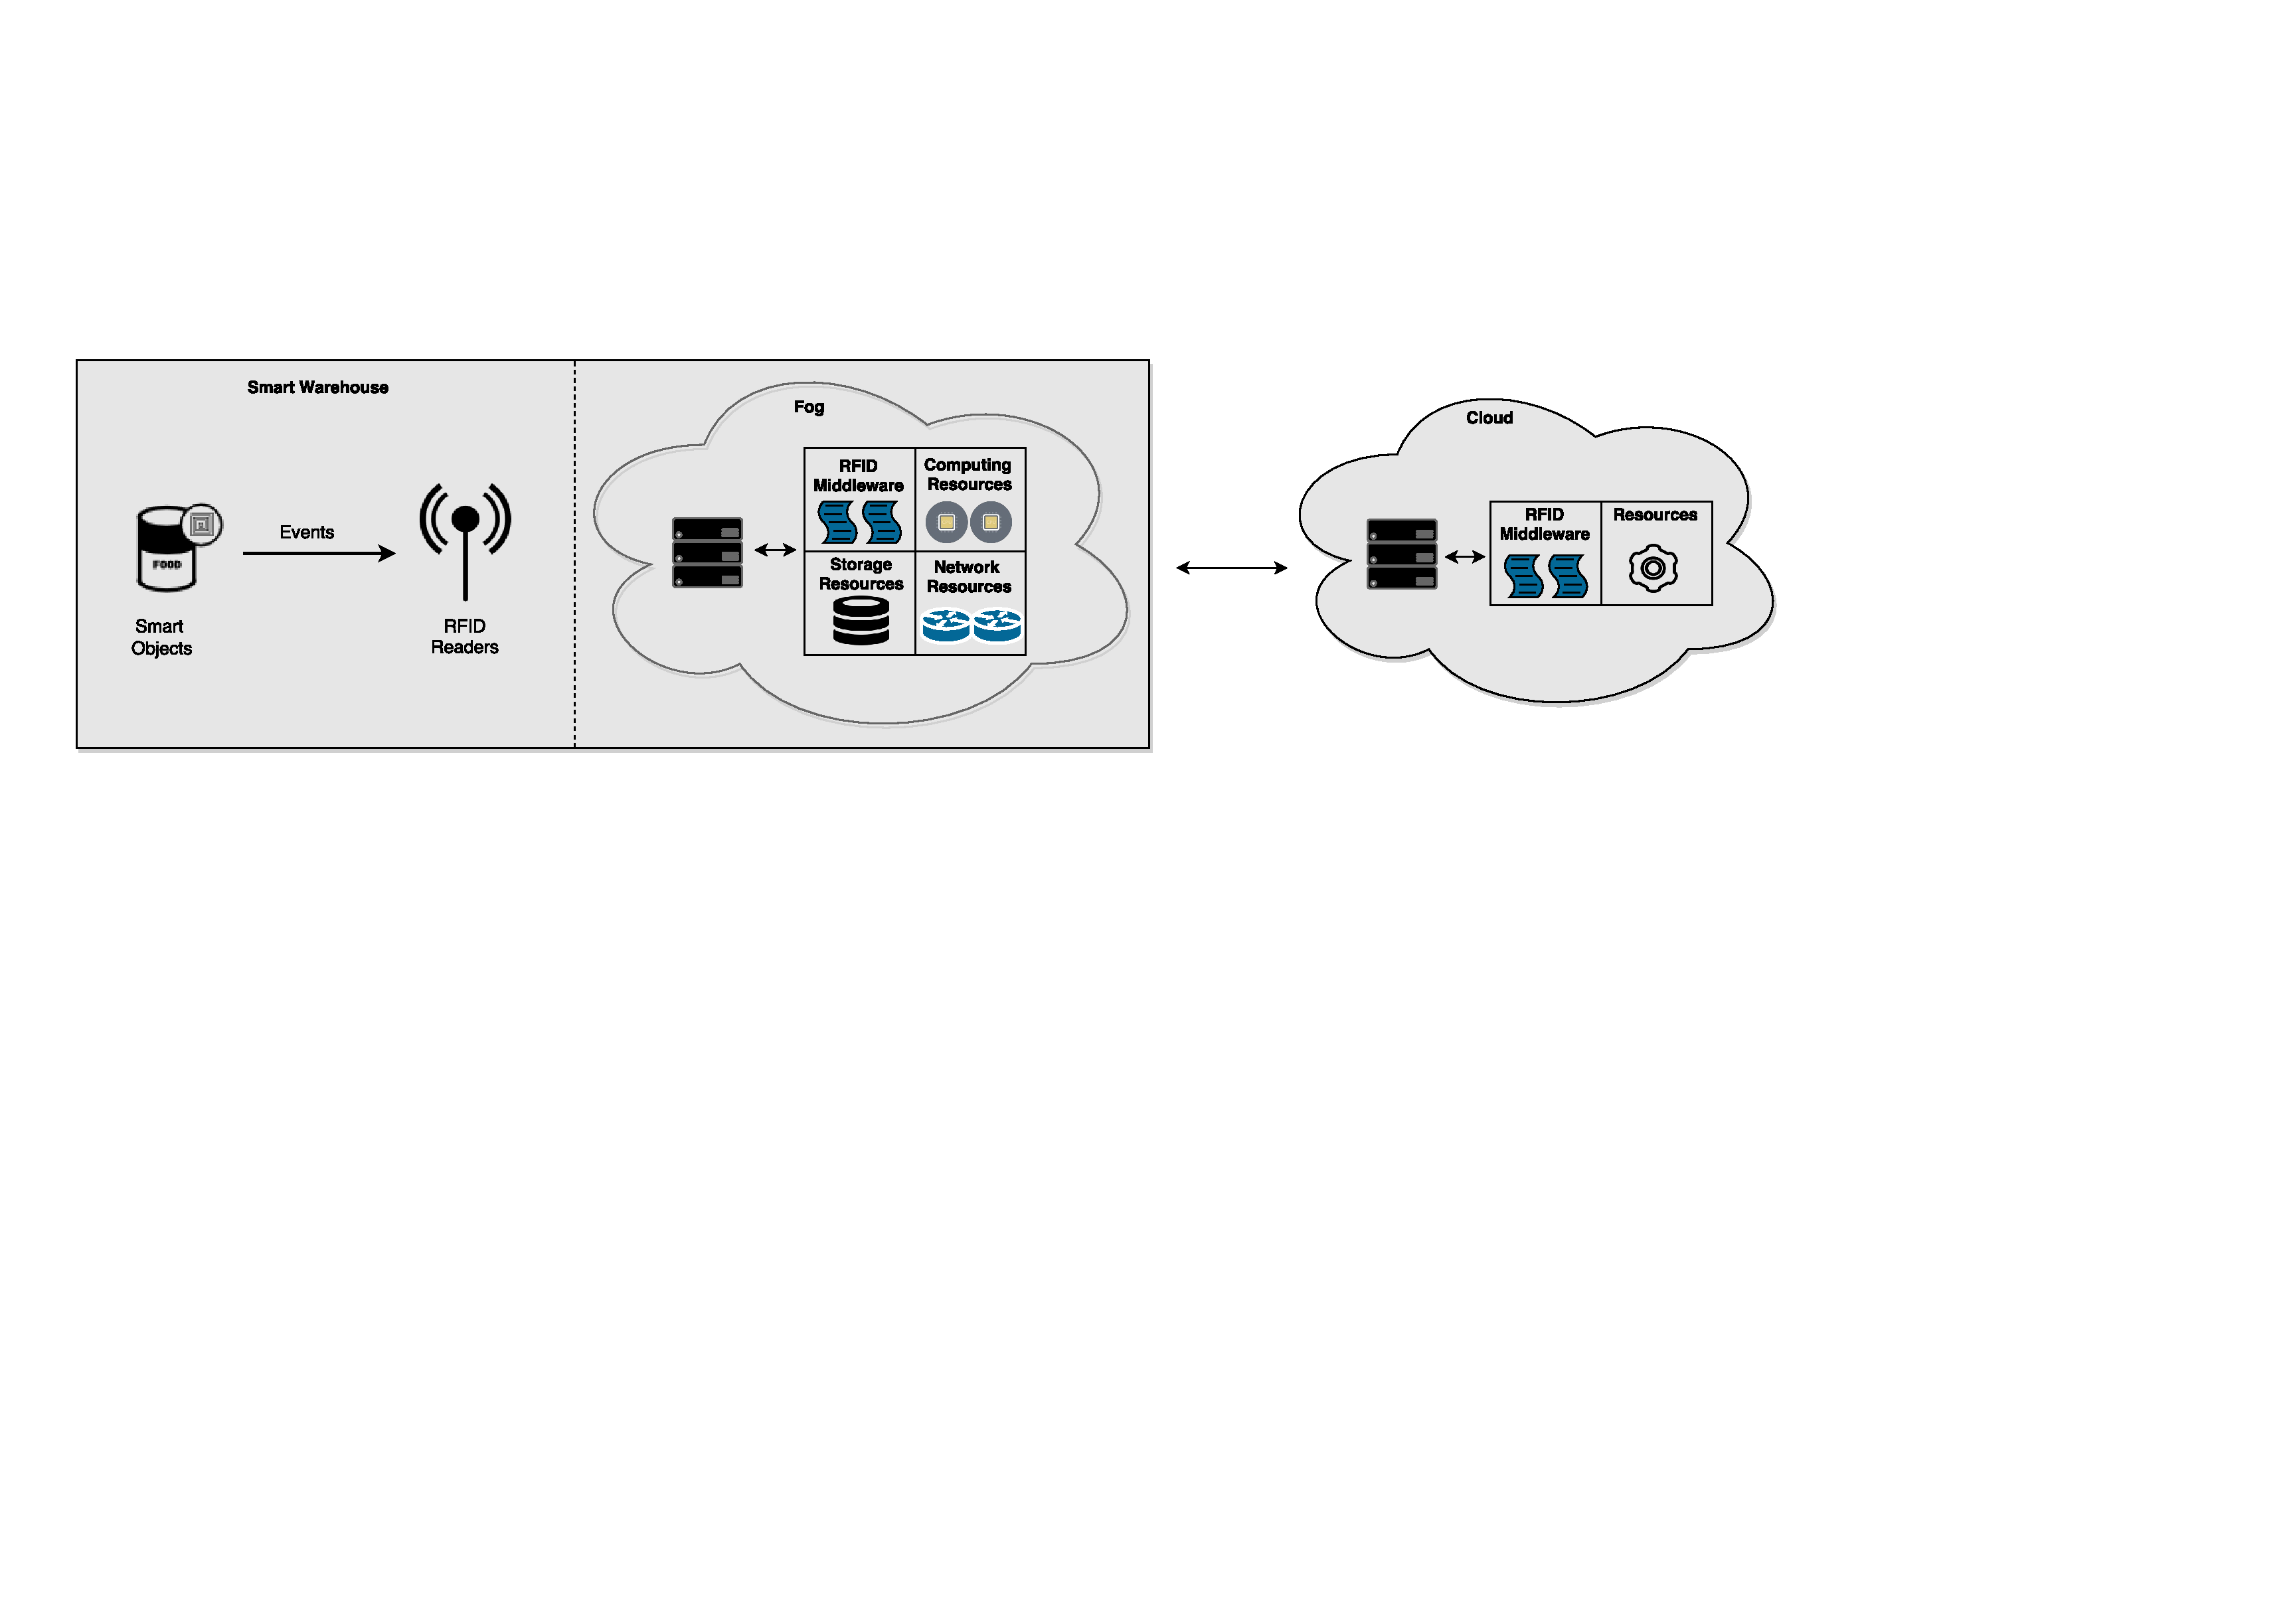
\includegraphics[width=\textwidth]{./images/solution_fog_architecture}
  \caption{Fog-approach: smart warehouse conceptual architecture.}
  \label{fig:solution_fog_architecture}
\end{figure}

Figure~\ref{fig:solution_fog_architecture} presents the architecture of a fog-based smart warehouse.
As in the cloud-based approach the warehouse is composed of smart objects, sensors and readers.
The proposed approach aims to extend the cloud paradigm to the edge of the network. The fog achieves
that by virtualizing computing, storage and network resources.\\

Regarding the application middleware, the components are distributed across the cloud and
the fog. The application components that are responsible to store the data during a long period of
time are provisioned in the cloud. The components that are responsible to perform real-time processing
of the data generated in the warehouse, and the components that filter the data that is consumed
locally and must be delivered to the cloud are provisioned in the fog.\\

The smart warehouse can be connected to the fog through several types of connection, from a physical
connection to a wireless connection such as Wi-Fi, 3G or \gls{LTE}. The fog is connected to the cloud
usually through a wireless connection, usually a Wi-Fi connection.

% Provisioning
\section{Provisioning}
\label{sec:provisioning}
Here we propose a mechanism that automates the provisioning of software for \gls{IoT} applications
in the cloud. Our solution relies on configuration management tools that leverage existing software
stacks. Figure~\ref{fig:provisioning_generic_architecture} presents the architecture for the proposed
mechanism.\\

% Provisioning mechanism conceptual architecture
\begin{figure}[ht!]
  \centering
  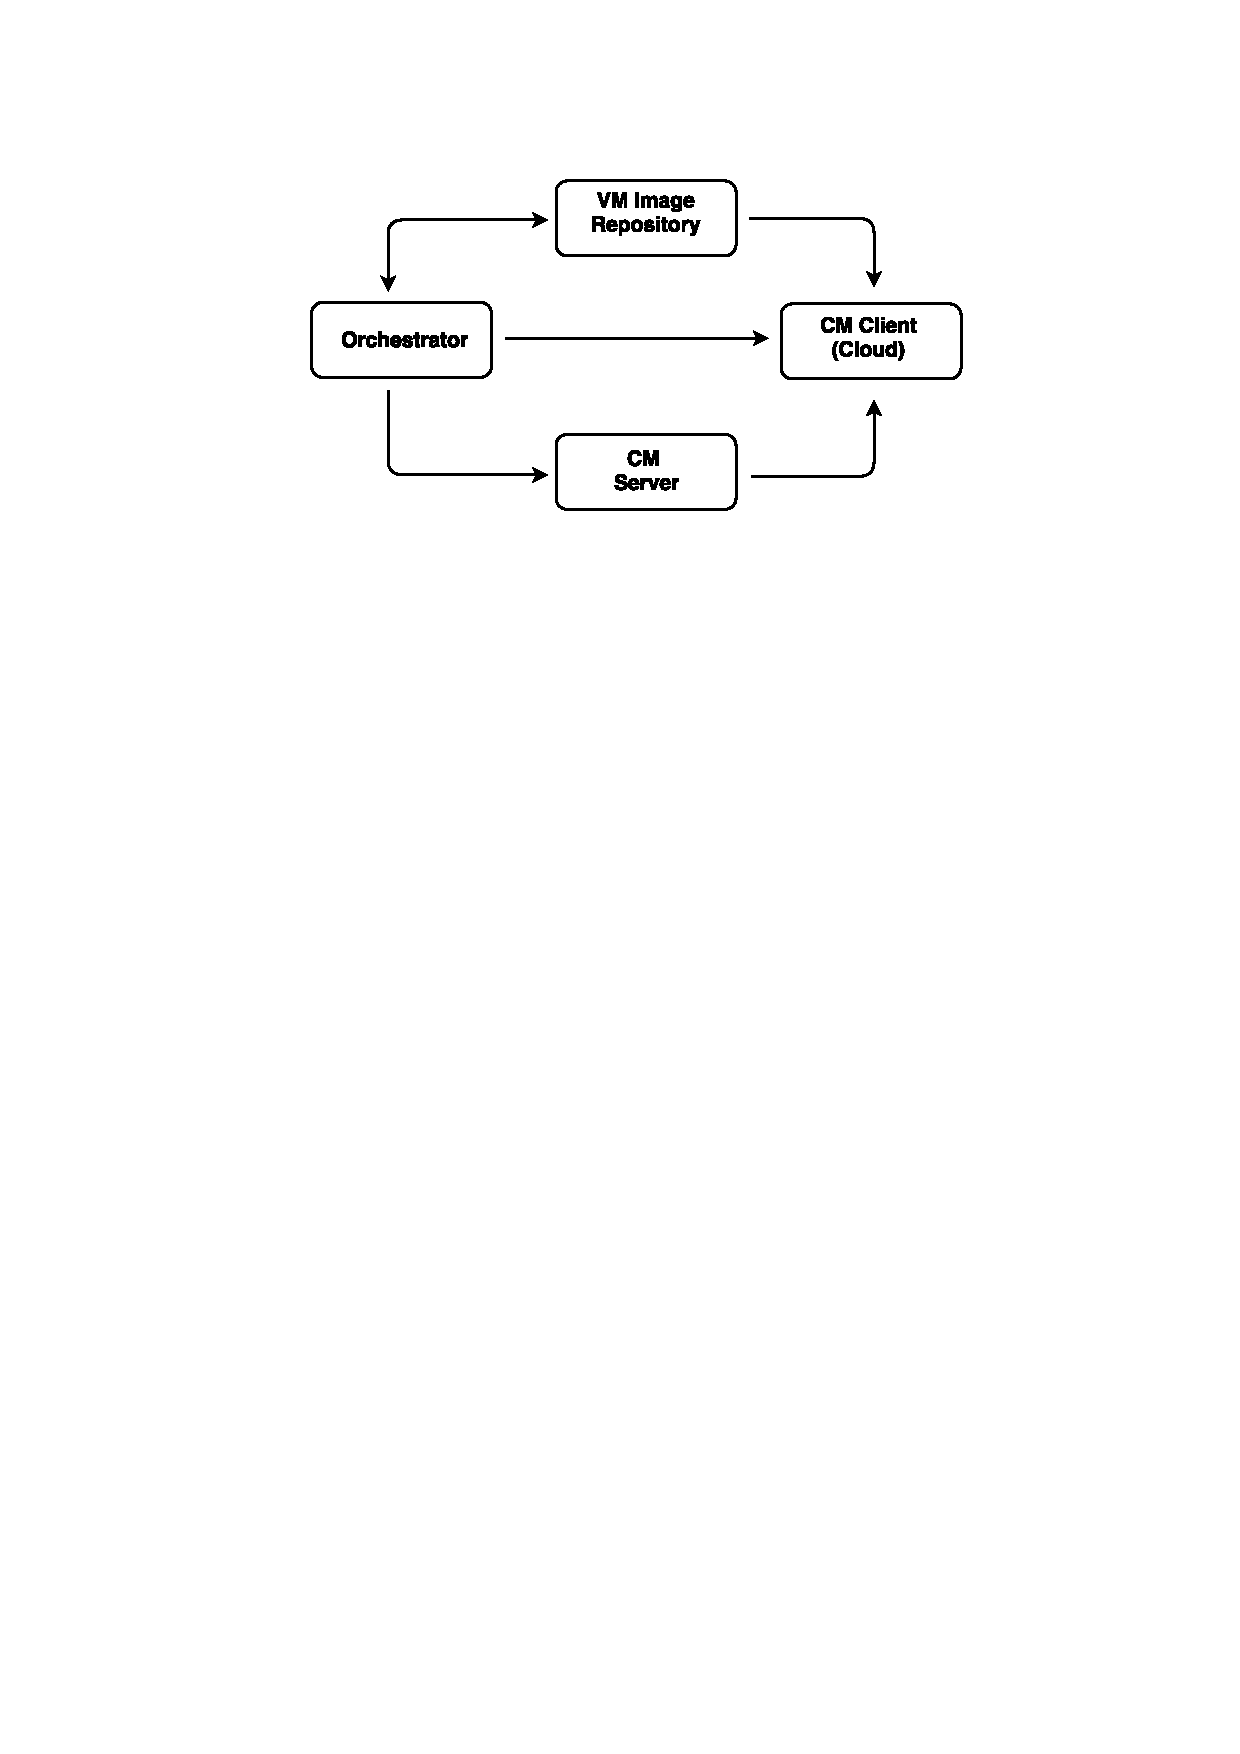
\includegraphics[width=.7\textwidth]{images/c4t-generic-solution.pdf}
  \caption{Provisioning mechanism conceptual architecture.}
  \label{fig:provisioning_generic_architecture}
\end{figure}

In our architecture, the provisioning policies and software images of a smart place are defined and
configured in a local environment and then uploaded to its respective repositories. When the provisioning
request is performed - through a configuration management interface in a local environment - the
configuration management (CM) client in the server node pulls the polices from the configuration
management server, a centralized server that is responsible to maintain a consistent state of the
provisioned nodes in the cloud. In order to enforce the polices, the CM client pulls the software
images from a central repository and then performs the provisioning and configuration of the software.
After provisioning the infrastructure the CM client periodically polls the CM server in order to
determine if its current state is consistent with the most recent policy.
